\documentclass[15pt]{beamer}

\usetheme{metropolis}
\usepackage{appendixnumberbeamer}

\usepackage{booktabs}
\usepackage[scale=2]{ccicons}

\usepackage{pgfplots}
\usepgfplotslibrary{dateplot}

\usepackage{subcaption}
\usepackage{graphicx}

\usepackage{xspace}
\newcommand{\themename}{\textbf{\textsc{metropolis}}\xspace}

\definecolor{Blue}{HTML}{0087BD}
\definecolor{Orange}{HTML}{FF7538}

\setbeamercolor{alerted text}{fg=Orange}
\setbeamercolor{frametitle}{bg=Blue}


\title{Classifying different types of blood cells from microscopic images}
%\subtitle{A modern beamer theme}
\date{\today}
\author{Johannes Kollek \& Jean-Marco Alameddine}
\institute{Machine Learning for Physicists - TU Dortmund}
% \titlegraphic{\hfill\includegraphics[height=1.5cm]{logo.pdf}}

\begin{document}

\maketitle

% \begin{frame}{Table of contents}
%   \setbeamertemplate{section in toc}[sections numbered]
%   \tableofcontents[hideallsubsections]
% \end{frame}

%\section{Introduction}
% 
% \begin{frame}[fragile]{Metropolis}

%   The \themename theme is a Beamer theme with minimal visual noise
%   inspired by the \href{https://github.com/hsrmbeamertheme/hsrmbeamertheme}{\textsc{hsrm} Beamer
%   Theme} by Benjamin Weiss.

%   Enable the theme by loading

%   \begin{verbatim}    \documentclass{beamer}
%     \usetheme{metropolis}\end{verbatim}

%   Note, that you have to have Mozilla's \emph{Fira Sans} font and XeTeX
%   installed to enjoy this wonderful typography.
% \end{frame}
% \begin{frame}[fragile]{Sections}
%   Sections group slides of the same topic

%   \begin{verbatim}    \section{Elements}\end{verbatim}

%   for which \themename provides a nice progress indicator \ldots
% \end{frame}

%\section{Title formats}

\begin{frame}{Problem}
    \begin{itemize}
      \setlength\itemsep{1em}
      \item The task is to distinguish between four different types of white blood cells from microscopic blood test images
      \item Couting blood cells is an important task in diagnosing diseases
      \item Manual classification requires technical knowledge and is very time-consuming
      \item[$\Rightarrow$] Machine Learning provides and efficient and fast method to solve this task
    \end{itemize}
\end{frame}


{
\begin{frame}{Dataset}
  \begin{itemize}
    \item Dataset found on Kaggle, published on \url{https://github.com/Shenggan/BCCD_Dataset} \newline (MIT license)
    \item $\approx 12500$ images including a white blood cell
    \item Colored $320 x 240$ pixels images
    \item Four different labels charaterizing the cell (Eosinophil, Lymphocyte, Monocyte, Neutrophil)
    \item Two kaggle kernels dealing with this specific dataset
    \item Several papers addressing this problem (with different datasets)

  \end{itemize}
\end{frame}
}

{


{
\begin{frame}{Example images from the dataset}
\begin{figure}
  \begin{subfigure}[t]{.4\textwidth}
    \centering
    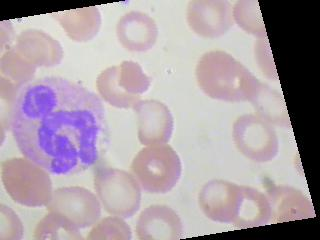
\includegraphics[width=\linewidth]{neutrophil.jpeg}
    \caption{Neutrophil.}
  \end{subfigure}
  \hfill
  \begin{subfigure}[t]{.4\textwidth}
    \centering
    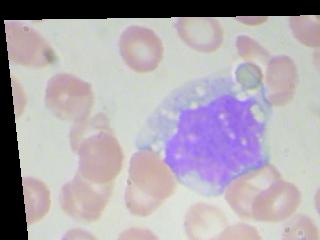
\includegraphics[width=\linewidth]{monocyte.jpeg}
    \caption{Monocyte.}
  \end{subfigure}

  \medskip

  \begin{subfigure}[t]{.4\textwidth}
    \centering
    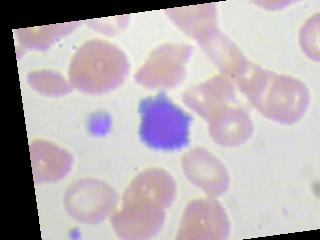
\includegraphics[width=\linewidth]{lymphocyte.jpeg}
    \caption{Lymphocyte.}
  \end{subfigure}
  \hfill
  \begin{subfigure}[t]{.4\textwidth}
    \centering
    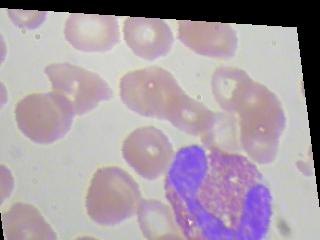
\includegraphics[width=\linewidth]{eosinophil.jpeg}
    \caption{Eosinophil.}
  \end{subfigure}
\end{figure}


\end{frame}
}


\begin{frame}{Alternative methods}
    \begin{itemize}
      \setlength\itemsep{1em}
      \item Using alternative methods to solve the problem...
      \item ... but the question is: ARE there any alternative methods that are applicable to this problem? \newline (Without using an enormous amount of preprocessing)
    \end{itemize}
\end{frame}

\end{document}
